\documentclass[main.tex]{subfiles}
\begin{document}
\section{Problem Set 10}
\subsection{Problem 1}
\begin{claim}
    Let $A \subseteq \RR^n$, $\vf : A \to \RR^m$. Suppose $\limv{a} \vf\parens{\vx}$ exists. Let $\braces{\vseq{x}}_{k = 1, 2, \ldots}$ be $\parens{A\setminus \braces{\va}}$-valued and $\limk \vseq{x} = \va$. Prove $\limk \vf\parens{\vseq{x}} = \limv{a} \vf\parens{\vx}$.
\end{claim}

\begin{soln}
    Let $\vg : A \to \RR$ be a function continuous at $\va$ satisfying $\vg =     \vf\parens{\vx}$ for all $\vx \in A \setminus \braces{\va}$. Observe that
    \begin{align*}
        \limv{a} \vf\parens{\vx} &= \limv{a} \vf|_{A\setminus\braces{\va}} \parens{\vx} \\
        &= \limv{a} \vg|_{A\setminus\braces{\va}} \parens{\vx} \\
        &= \limv{a} \vg\parens{\vx} \\
        &= \vg\parens{\va} \\
        &= \limk \vg\parens{\vseq{x}},
    \end{align*}
    where the last equality comes from the converse of Problem Set 7 Problem 3. Since $\vseq{x} \neq \va$ for all $k\in \NN$, we have $\limk \vf\parens{\vseq{x}} = \limk \vg\parens{\vseq{x}} = \limv{a}\vf\parens{\vx}$ as desired.
\end{soln}
\eject

\subsection{Problem 2}
\begin{claim}
    Let $A \subseteq \RR^n$, $\vf : A \to \RR^m$. Suppose $\limv{a} \vf\parens{\vx}$ exists. Let $\sigma > 0$, $\gamma : [0, \sigma)\to \RR^n$ be continuous, $\gamma\parens{0} = \va$, and $\gamma\parens{\parens{0, \sigma}} \subseteq A\setminus \braces{\va}$. Prove $\lim_{t\to 0}\vf\parens{\gamma\parens{t}} = \limv{a}\vf\parens{\vx}$.
\end{claim}

\begin{soln}
    Let $\vg : A \to \RR$ be a function continuous at $\va$ satisfying $\vg =     \vf\parens{\vx}$ for all $\vx \in A \setminus \braces{\va}$. Since $\gamma$ is continuous at $0$ and $\vg$ is continuous at $\gamma(0) = \va$, we know that $\vg\circ\gamma : [0, \sigma) \to \RR^m$ is continuous at $0$; thus, 
    \begin{align*}
        \lim_{t\to 0} \vf\parens{\gamma(t)} &= \lim_{t\to 0} \vg\parens{\gamma(t)} \\
        &= \vg\parens{\gamma(0)} \\
        &= \vg\parens{\va} \\
        &= \limv{a} \vg\parens{\vx} \\
        &= \limv{a} \vg|_{A\setminus\braces{\va}} \parens{\vx} \\
        &= \limv{a} \vf|_{A\setminus\braces{\va}} \parens{\vx} \\
        &= \limv{a} \vf\parens{\vx}
    \end{align*}
    as desired.
\end{soln}
\eject

\subsection{Problem 3}
\begin{claim}
    Let $U \subseteq \RR^n$ be open, $\vf : U \to \RR^m$ be differentiable at $\va \in U$, $\sigma > 0$, $\gamma: \parens{-\sigma,\sigma} \to \RR^n$ be differentiable at 0 with $\gamma\parens{0} = \va$ and $\gamma\parens{\parens{-\sigma,\sigma}} \subseteq U$. Prove $\parens{\vf \circ \gamma }'\parens{0} = \parens{\mathcal{D}_{\gamma'\parens{0}}\vf}\parens{\va}$
\end{claim}

\begin{soln}
    By the Chain Rule, $\parens{\vf \circ \gamma }'\parens{0} = \mathcal{D}\vf\parens{\gamma(0)} \mathcal{D}\gamma\parens{0} = \mathcal{D}\vf\parens{\va} \gamma'\parens{0}$. Since $\gamma$ is a function with domain $\parens{-\sigma, \sigma} \subseteq \RR$, it follows that $\gamma'\parens{0}$ is an $n\times 1$ matrix, or a vector in $\RR^n$; thus, $\mathcal{D}\vf\parens{\va} \gamma'\parens{0} = \parens{\mathcal{D}_{\gamma'\parens{0}}\vf}\parens{\va} \implies \parens{\vf \circ \gamma }'\parens{\va} = \parens{\mathcal{D}_{\gamma'\parens{0}}\vf}\parens{\va}$ as desired.
\end{soln}
\eject

\subsection{Problem 4}
\begin{claim}
    Consider the function $f : \RR^n \to \RR$ given by $f\parens{\vx} = \norm{\vx}$. Prove that $f$ is differentiable on $\RR^n\setminus \braces{\vec{0}}$ and not differentiable at $\vec{0}$. For $\vx \in \RR^n\setminus\braces{\vec{0}}$, prove that $\nabla f\parens{\vx} = \norm{\vx}^{-1}\vx$ in two ways. First, by computing the partial derivatives $\mathcal{D}_jf\parens{\vx}$ and showing they equal $x_j/\norm{\vx}$ in case $\vx = \parens{x_1,\ldots ,x_n}^\top$. Second, using the chain rule on $\norm{\vx} = \sqrt{\vx \cdot \vx}$, with facts from Problem Sets 8 and 9.
\end{claim}

\begin{soln}
    First we will show that $f$ is differentiable on $\RR^n\setminus\braces{\vec{0}}$ and not differentiable at $\vec{0}$. Observe that $f$ is equal to the composition of the square root function and $g: \RR^n \to \RR$ defined by $g(x_1, \ldots , x_n)^\top = \sum_{k = 1}^n x_k^2 \ge 0$. Since $g$ is a polynomial, it is differentiable; furthermore, restricting the domain of $g$ to $\RR^n\setminus\braces{\vec{0}}$, it will always return a positive real number since the equality case of $g(x_1, \ldots , x_n)^\top = 0$ is reached if and only if $(x_1, \ldots , x_n)^\top = \vec{0}$. In particular, we know that the square root function is differentiable on $\RR^+$ (by Problem Set 9 Problem 8), so $f$ is differentiable on $\RR^n\setminus \braces{\vec{0}}$ too by the chain rule.

    Next, observe that since $\sqrt{x}$ is not differentiable at $x = 0$, $\sqrt{g\parens{x_1, \ldots , x_n}^\top}$ cannot be differentiable at $g\parens{\vec{0}} = 0$, so $\norm{x}$ is not differentiable at $\vec{0}$ either. 

    Now we will show that $\nabla f\parens{\vx} = \norm{\vx}^{-1}\vx$. For $\vx = (x_1, \ldots , x_n)^\top \in \RR^n \setminus\braces{\vec{0}}$, we have by single-variable calculus that
    \[\pdv{}{x_j}\norm{\vec{x}} = \pdv{}{x_j}\sqrt{\sum_{k = 1} x_k^2} = \frac{1}{2\sqrt{\sum_{k = 1} x_k^2}} \cdot 2x_j = \frac{x_j}{\norm{\vx}}.\]
    Thus, $\nabla f\parens{\vx} = \parens{\frac{x_1}{\norm{\vx}}, \ldots , \frac{x_n}{\norm{\vx}}}^\top = \frac{1}{\norm{\vx}}\parens{x_1, \ldots , x_n}^\top = \frac{\vx}{\norm{\vx}}$ as desired.

    On the other hand, we have $\norm{\vx} = \sqrt{\norm{\vx}^2}$, so we also have
    \begin{align*}
        \nabla f\parens{\vx} &= \parens{\mathcal{D}\sqrt{\norm{\vx}^2}}^\top \\
        &= \parens{\frac{1}{2\sqrt{\norm{\vx}^2}}\cdot 2\vx^\top}^\top \\
        &= \frac{1}{\norm{\vx}}\vx
    \end{align*}
    as desired.
    
\end{soln}
\eject

\subsection{Problem 5}
\begin{claim}
    Consider the function $\vf : \RR^n \to \RR$ given by $f\parens{\vx} = \norm{\vx}$. Let $n = 2$ and $\vx = \parens{x_1,x_2}^\top \in \RR^2 \setminus \braces{0}$. Note that $\vx$ lies on the circle of radius $r = \norm{x} > 0$ centered at the origin of $\RR^2$. In what unit direction(s) $\vec{v} = \parens{v_1,v_2}^\top$ would you nudge $\vx$ to increase its distance from the origin the fastest? Slowest? Stay infinitesimally constant (i.e., $\mathcal{D}_{\vec{v}}f\parens{\vx} = 0$)? Draw a schematic picture.
\end{claim}

\begin{soln}
    I would nudge $\vx$ in the unit direction of $\frac{1}{\norm{\vx}}\vx$ to increase its distance from the origin the fastest; this is justified by the fact that $\max\braces{\mathcal{D}_{\vec{v}}f\parens{\vx} \mid \vec{v} \in \RR^n , \norm{\vec{v}} = 1}$ is achieved when $\vec{v} = \frac{1}{\norm{\nabla f\parens{\vx}}} \nabla f\parens{\vx} = \frac{1}{\norm{\vx}}\vx$ due to the previous problem; similarly, I would nudge $\vx$ in the unit direction of $-\frac{1}{\norm{\vx}}\vx$ to increase its distance from the origin the slowest. Intuitively, this can be thought of as extending/shrinking the straight line from the origin to $\vx$ as the most/least efficient way to increase the distance.
    
    On the other hand, to stay infinitesimally constant, I would pick $\vec{v}$ so that it is perpendicular with $\vx$; this way, $\vec{v}$ is essentially on the tangent line from the circle of radius $\norm{\vx}$, i.e. it is the ``best" approximation of $\norm{\vx}$ using single-variable calculus.
    \begin{center}
        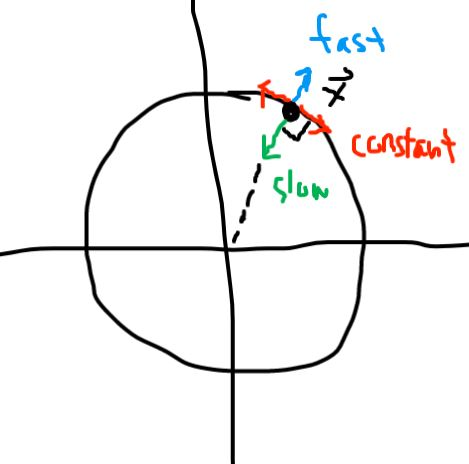
\includegraphics[width = 0.5\textwidth]{pset9p5.JPG}
    \end{center}
\end{soln}
\eject

\subsection{Problem 6}
\begin{claim}
    Consider the function $\vh : \RR^2 \to \RR^2$ given by $\vh\parens{\parens{x_1,x_2}^\top} = \parens{x_1^2 + x_2^2,x_1^2 - x_2^2}^\top$. Note that it can be viewed as the composition $f \circ g$ where $f : \RR^2 \to \RR^2$ is $f\parens{\parens{y_1,y_2}^\top} = \parens{y_1 + y_2,y_1 - y_2}^\top$ and $g : \RR^2 \to \RR^2$ is $g\parens{\parens{x_1,x_2}^\top} = \parens{x_1^2,x_2^2}^\top$ . Explain the differentiability of these functions. Compute $\mathcal{D}\vf\parens{\parens{1,1}^\top}$, $\mathcal{D}\vg\parens{\parens{1,-1}^\top}$, and $\mathcal{D}\vh\parens{\parens{1,-1}^\top}$ directly. Verify that we have $\mathcal{D}\vh\parens{\parens{1,-1}^\top} = \mathcal{D}\vf\parens{\parens{1, 1}^\top}\mathcal{D}\vg\parens{\parens{1,-1}^\top}$ (as the chain rule predicts) by doing out the matrix multiplication.
\end{claim}

\begin{soln}
    First, note that $\vf$, $\vg$, and $\vh$ are both polynomials in $\RR^2$, so they are differentiable. Next, observe that
    \begin{align*}
        \mathcal{D}\vf\parens{\parens{x_1, x_2}^\top} &= \begin{pmatrix}
            \pdv{}{x_1} x_1 + x_2 & \pdv{}{x_2} x_1 + x_2 \\
            \pdv{}{x_1} x_1 - x_2 & \pdv{}{x_2} x_1 - x_2
        \end{pmatrix} \\
         &= \begin{pmatrix}
            1 & 1 \\
            1 & -1
        \end{pmatrix} \\
        &\implies \mathcal{D}\vf\parens{\parens{1, 1}^\top} = \begin{pmatrix}
            1 & 1 \\
            1 & -1
        \end{pmatrix},
    \end{align*}
    \begin{align*}
        \mathcal{D}\vg\parens{\parens{x_1, x_2}^\top} &= \begin{pmatrix}
            \pdv{}{x_1} x_1^2 & \pdv{}{x_2} x_1^2 \\
            \pdv{}{x_1} x_2^2 & \pdv{}{x_2} x_2^2
        \end{pmatrix} \\
         &= \begin{pmatrix}
            2x_1 & 0 \\
            0 & 2x_2
        \end{pmatrix} \\
        &\implies \mathcal{D}\vg\parens{\parens{1, -1}^\top} = \begin{pmatrix}
            2 & 0 \\
            0 & -2
        \end{pmatrix},
    \end{align*}
    and
    \begin{align*}
        \mathcal{D}\vh\parens{\parens{x_1, x_2}^\top} &= \begin{pmatrix}
            \pdv{}{x_1} x_1^2 + x_2^2 & \pdv{}{x_2} x_1^2 + x_2^2 \\
            \pdv{}{x_1} x_1^2 - x_2^2 & \pdv{}{x_2} x_1^2 - x_2^2
        \end{pmatrix} \\
         &= \begin{pmatrix}
            2x_1 & 2x_2 \\
            2x_1 & -2x_2
        \end{pmatrix} \\
        &\implies \mathcal{D}\vh\parens{\parens{1, -1}^\top} = \begin{pmatrix}
            2 & -2 \\
            2 & 2
        \end{pmatrix}.
    \end{align*}
    Then we have
    \begin{align*}
        &\begin{pmatrix}
            2 & -2 \\
            2 & 2
        \end{pmatrix} = \begin{pmatrix}
            1\cdot 2 + 1\cdot 0 & 1\cdot 0 + 1\cdot (-2) \\
            1\cdot 2 + (-1)\cdot 0 & 1\cdot 0 + (-1)\cdot (-2)
        \end{pmatrix} = \begin{pmatrix}
            1 & 1 \\
            1 & -1
        \end{pmatrix} \begin{pmatrix}
            2 & 0 \\
            0 & -2
        \end{pmatrix} \\
        &\implies \mathcal{D}\vh\parens{\parens{1,-1}^\top} = \mathcal{D}\vf\parens{\parens{1, 1}^\top}\mathcal{D}\vg\parens{\parens{1,-1}^\top}
    \end{align*}
    as desired.
\end{soln}
\eject

\subsection{Problem 7}
\begin{claim}
    Prove that $U = \set*{\parens{x,y}^\top \in \RR^2 \mid y \neq 0}$ is an open subset of $\RR^2$.
\end{claim}

\begin{soln}
    Let $(x, y)^\top \in U$. Let $(x_1, y_1)^\top \in B_{\frac{\abs{y}}{2}}\parens{(x, y)^\top}$; then by definition
    \begin{align*}
        &\norm{(x_1, y_1)^\top - (x, y)^\top} < \frac{\abs{y}}{2} \\
        &\implies \sqrt{(x - x_1)^2 + (y - y_1)^2} < \frac{\abs{y}}{2} \\
        &\implies (x - x_1)^2 + (y - y_1)^2 < \frac{y^2}{4}.
    \end{align*}
    If $y_1 = 0$, then $(x - x_1)^2 + (y - y_1)^2 = (x - x_1)^2 + y^2 \ge y^2$; however, $y^2 > \frac{y^2}{4}$, contradiction! Thus, $(x_1, y_1)^\top\in U\implies B_{\frac{\abs{y}}{2}}\parens{(x, y)^\top} \subseteq U$, so we're done.
\end{soln}
\eject

\subsection{Problem 8}
\begin{claim}
    With $U$ as above, consider the function $f : U \to \RR$ given by $f\parens{\parens{x,y}^\top} = x^3/y$. Explain why $f$ is differentiable on $U$ and compute $\nabla f\parens{\parens{x,y}^\top}$.
\end{claim}

\begin{soln}
    Since $f$ is the quotient of two polynomials on $U$ (with the denominator $y$ always being nonzero by definition of $U$), which themselves are differentiable on $U$, the quotient rule guarantees that $f$ is differentiable. We also have
    \[\nabla f\parens{\parens{x,y}^\top} = \begin{pmatrix}
        \pdv{}{x} f\parens{\parens{x, y}^\top} \\
        \pdv{}{y} f\parens{\parens{x, y}^\top}
    \end{pmatrix} = \begin{pmatrix}
        \pdv{}{x} \frac{x^3}{y} \\
        \pdv{}{y} \frac{x^3}{y}
    \end{pmatrix} = \boxed{\begin{pmatrix}
        \frac{3x^2}{y} \\
        -\frac{x^3}{y^2}
    \end{pmatrix}}.\]
\end{soln}
\eject

\subsection{Problem 9}
\begin{claim}
    Prove the $C^1$ version of the chain rule: if $U \subset \RR^n$, $V \subset \RR^m$ are open, $\vg : U \to \RR^m$ is $C^1$ on $U$, $\vf : V \to \RR^p$ is $C^1$ on $V$, and $\vg\parens{U} \subseteq V$, then $\vf \circ \vg : U \to \RR^p$ is $C^1$ on $U$.
\end{claim}

\begin{soln}
    If $\vf$ is $C^1$ on $V$, then by definition $\mathcal{D}_j \vf$ exists and is continuous for all $j\in \braces{1, \ldots , m}$; similarly, $\mathcal{D}_j \vg$ exists and is continuous for all $j\in \braces{1, \ldots , n}$. Furthermore, both $\vf$ and $\vg$ must then be differentiable (and by extension continuous). It suffices to show that for any $\vx \in U$, $\parens{\mathcal{D}_j \vf\circ \vg}\parens{\vx}$ exists and is continuous for all $j\in \braces{1, \ldots , m}$. 
    
    Observe that the former is clearly true since $\vf$ and $\vg$ being $C^1$ implies that they are differentiable at $\vg\parens{\vx}$ and $\vx$ respectively, and therefore that their composition is differentiable at $\vx$ as well, so the partial derivatives of $\vf\circ\vg$ at $\vx$ are just each of the column vectors of $\parens{\mathcal{D} \vf\circ \vg}\parens{\vx}$.
    
    Next, observe that by the Chain Rule,
    \[\parens{\mathcal{D}_j\vf\circ \vg}\parens{\vx} = \parens{\mathcal{D}\vf\circ \vg}\parens{\vx}\vec{e}_j = \parens{\parens{\mathcal{D}\vf}\parens{\vg\parens{\vx}} \mathcal{D}\vg\parens{\vx}}\vec{e}_j = \underbrace{\parens{\mathcal{D}\vf}\parens{\vg\parens{\vx}}}_{p\times m \text{ matrix}} \underbrace{\mathcal{D}_j\vg\parens{\vx}}_{m\times 1 \text{ matrix}}.\]
    Let $\parens{\mathcal{D}\vf}\parens{\vg\parens{\vx}} = \begin{pmatrix}
        \parens{\mathcal{D}_1\vf_1}\parens{\vg\parens{\vx}} & \ldots & \parens{\mathcal{D}_m\vf_1}\parens{\vg\parens{\vx}} \\
        \vdots & \ddots & \vdots \\
        \parens{\mathcal{D}_1\vf_p}\parens{\vg\parens{\vx}} & \ldots & \parens{\mathcal{D}_m\vf_p}\parens{\vg\parens{\vx}}
    \end{pmatrix},\mathcal{D}_j\vg\parens{\vx} = \begin{pmatrix}
        \mathcal{D}_j\vg_1\parens{\vx} \\
        \vdots \\
        \mathcal{D}_j\vg_m\parens{\vx}
    \end{pmatrix}$. Then
    \[\parens{\mathcal{D}_j\vf\circ \vg}\parens{\vx} = \parens{\mathcal{D}\vf}\parens{\vg\parens{\vx}}\mathcal{D}_j\vg\parens{\vx} = \begin{pmatrix}
        \sum_{i = 1}^m \parens{\mathcal{D}_i\vf_1}\parens{\vg\parens{\vx}}\mathcal{D}_j\vg_i\parens{\vx} \\
        \vdots \\
        \sum_{i = 1}^m \parens{\mathcal{D}_i\vf_p}\parens{\vg\parens{\vx}}\mathcal{D}_j\vg_i\parens{\vx}
    \end{pmatrix}.\]
    Since $\mathcal{D}_j\vg\parens{\vx} : U \to \RR^m$ is continuous at $\vx$, this means that each of its components $\mathcal{D}_j\vg_k\parens{\vx} : U \to \RR$ are continuous at $\vx$ for $k = 1, \ldots , m$ by Problem Set 9 Problem 1. Similarly, since each of the functions $\parens{\mathcal{D}_\ell\vf}\circ \vg : U \to \RR^p$ are continuous at $\vx$ for $\ell = 1, \ldots , m$ as compositions of a continuous partial derivative $\mathcal{D}_\ell\vf$ with the continuous function $\vg$, this means that each of the functions' components $\parens{\mathcal{D}_\ell\vf_k}\circ \vg : U \to \RR$ are continuous at $\vx$ for $k = 1, \ldots , p$. In particular, this means that all of the components of $\parens{\mathcal{D}_j\vf\circ \vg}\parens{\vx}$ are continuous at $\vx$ since each component is the sum of products of continuous real-valued functions, so $\parens{\mathcal{D}_j\vf\circ \vg}\parens{\vx}$ itself must be continuous due to Problem Set 9 Problem 1. Thus, we've shown that $\vf \circ \vg$ is $C^1$ on $U$ as desired.
\end{soln}
\eject

\subsection{Problem 10}
\begin{claim}
    Prove that if $\varphi : \RR \to  \RR$ is $C^1$ and $g\parens{\vx} = \varphi\parens{\norm{\vx}}$ for $\vx \in \RR^n$, then $g$ is $C^1$ on $\RR^n \setminus \braces{\vec{0}}$ and $\mathcal{D}_j g\parens{\vx} = \frac{x_j}{\norm{\vx}}\varphi'\parens{\norm{\vx}}$ for all $\vx \neq \vec{0}$.
\end{claim}

\begin{soln}
    Let $\vf\parens{\vx} = \norm{\vx}$. First, we will show that $\vf$ is $C^1$ on $\RR$. Recall from Problem 4 that $\mathcal{D}_j\vf\parens{\vx} = \frac{x_j}{\norm{\vx}}$ for each $j = 1, \ldots , n$; since $\norm{\vx}$ is continuous as a corollary of Problem Set 9 Problem 9 (taking $\vg\parens{\vx} = \vx$, which itself is continuous by Problem Set 8 Problem 9) and $x_j$ is continuous as a polynomial, we get that $\mathcal{D}_j\vf\parens{\vx}$ must be continuous too (as $\vx\in \RR^n\setminus\braces{\vec{0}}\implies \norm{\vx} \neq 0$). By the previous problem, this implies that $g$ is $C^1$ on $\RR^n\setminus\braces{\vec{0}}$. Thus, by the Chain Rule, we find that if $\vx\neq \vec{0}$, then
    \[\mathcal{D}_jg\parens{\vx} = \mathcal{D} \varphi\parens{\vf\parens{\vx}} \mathcal{D}_j\vf\parens{\vx} = \varphi'\parens{\vf\parens{\vx}} \frac{x_j}{\norm{\vx}} = \frac{x_j}{\norm{\vx}}\varphi'\parens{\norm{\vx}}\]
    as desired.
\end{soln}
\eject

\end{document}